\chapter{Pushdown automata and parsing}
	Pushdown automaton: a finite state machine enriched with a LIFO queue (or \emph{stack}) as memorization device, that supports the classical push-pop operations. 
	It's useful to portay this device with a terminator on the bottom, so that it signals the emptiness of the stack. Even a single-state nondeterministic pushdown 
	automaton can (with only the stack) be used as a recognizer; this is called \emph{daisy automaton}.

	To define a pushdown automaton we just expands the FSA deefinition with the stack alphabet and a special character from this alphabet, the stack bottom / terminator 
	/ initial stack symbol. REMEMBER: the transiction function doeas not depends solely on the given input anymore, but also on the stack's top symbol; the domain is 
	changed, wrt the classic FSA.

	Domain and range of the transiction function for a FSA: (set of states) $\times$ (input alphabet) $\rightarrow$ (set of states)

	Domain and range of the transiction function for a PDA: (set of states) $\times$ (input alphabet) $\times$ (stack alphabet) $\rightarrow$ (set of states) 
	$\times$ (stack alphabet)

	In the graph for a pushdown automaton, also the stack operation must be specified.
	\textbf{\underline{A pushdown automaton is as expressive as a context free grammar}}
	
	\section{Deterministic stuff}
		Only deterministic context free languages (so, accepted by deterministic PDA) are considered in the field of compilers, due to efficiency and complexity 
		reasons.

		Non determinism can be found in PDA in 2 forms mainly:
		\begin{itemize}
			\item the transiction function is multi valued (it has more than one possible output for certain input)
			\item spontaneous moves \emph{interfere} with the recognizing procedure, in particular
				\begin{itemize}
					\item a spontaneous move and a reading move are defined and they overlap
					\item a spontaneous move is multi-valued
				\end{itemize}
		\end{itemize}
		
		\subsection{Deterministic languages family}
			The DET family (the context free languages that can be recognized by a deterministic PDA) is a proper subset of the CF languages family.

			This family is closed under these operators:
			\begin{figure}[htp]
				\begin{center}
					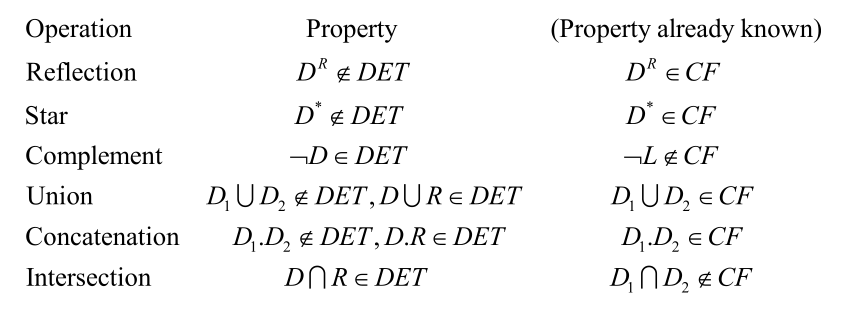
\includegraphics[width = \textwidth]{./images/detClosures.png}
					\caption{Closures properties of deterministic languages}
				\end{center}
			\end{figure}
	
	\section{Parsing}
		Parsing (syntax analysis) is the procedure to estabilish if a string belongs to a certain language. A parser is an automaton that puts in place the analysis. 
		It compute the syntax trees or gives an error if it finds one.
		
		\subsubsection{Types of parsing}
			Parsers can be classified in top-down parsers and bottom-up parsers (another distinction that's totally new to CS students, uh?) to distinguish between 
			the approach to the syntax trees.
			\begin{itemize}
				\item \emph{top down} analyzers grow the tree from the root downwards towards the leaves; this means that every step of the algorithm corresponds to 
				a \emph{derivation in the grammar} so a \emph{left} $\rightarrow$ \emph{right} passage in a rule
				\item \emph{bottom up} parsers starts from the leaves of the syntax tree and reach the root; this means that every step of the parsing procedure 
				corresposnds to a \emph{reduction in the grammar}, so a \emph{right} $\rightarrow$ \emph{left} passage in a rule
			\end{itemize}
		
		\subsection{Grammars as networks of finite automata}
			To build a recognizer for a grammar, we can see it as a set of indipendent productions for each nonterminal. Every nonterminal is associated with a 
			dedicated machine (a FSA, for example) that when has to read another nonterminal just "invokes" another machine to do so.

			This means that, at the end of the transformation, we have a machine for every nonterminal, that can interpret all the productions of said nonterminal, 
			and on the arcs has all and only the right-side elements of the rule taken into account.
			
			\subsubsection{Good example}
				We consider a grammar that generates arithmetic expressions.
				\begin{figure}[htp]
					\begin{center}
						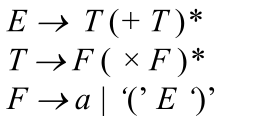
\includegraphics[]{./images/exGrammar.png}
					\end{center}
				\end{figure}
				We isolate the three nonterminals E, T and F and build a machine for each one of them
				\begin{figure}[htp]
					\begin{center}
						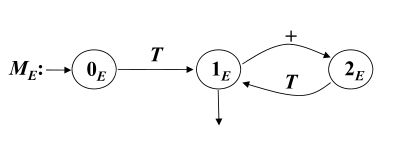
\includegraphics[]{./images/exE.png}
					\end{center}
				\end{figure}
				\begin{figure}[htp]
					\begin{center}
						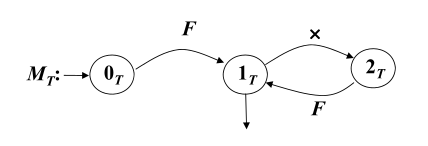
\includegraphics[]{./images/exT.png}
					\end{center}
				\end{figure}
				\begin{figure}[htp]
					\begin{center}
						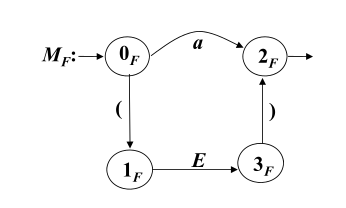
\includegraphics[]{./images/exF.png}
					\end{center}
				\end{figure}
				
		\subsection{Lookahead sets}
			All parsers are implemented as DPDA. They rely on a second component, the lexical analyzer, that reads the input stream and recognizes the patterns in it 
			in order to separate all the lexeme (or tokens) to give to the parser itself.

			To ensure the automaton is actually deterministic, parsers \emph{preprocess} the grammar's rules, and select the sets of tokens that can be read after 
			each move; these are the \emph{followers} or \emph{lookahead} set. These sets of token are useful when another machine in the network must be called: 
			it's necessary to know which character we \emph{will} read and compare it with the first character read in the machines. To be noted: each 
			\emph{nonterminal, for each configuration,} has a set of lookahead characters. 
			
			\subsubsection{Lookahead and closures}
				Each pair \{state, token\} is said to be a candidate if the token is a legal lookahed character for the current activation of the machine in state 
				"state". That does not mean so much, at the end of the day.

				To compute each set of candidates we use a \emph{closure function}. The closure function is defined this way:

				Let \emph{C} be a set of candidates:
				\begin{equation}
					\text{closure(\emph{C})} =
					\begin{cases}
				  		\text{\emph{C}} \\
				  		\langle 0_b, b \rangle \in \text{closure(\emph{C}) if }
				  		\begin{cases}
				  			\exists \text{ candidate } \langle q, a\rangle \in \text{\emph{C} \textbf{and}}\\
				  			\exists \text{ arc in the machine net so that } q \xrightarrow{B} r \text{\textbf{ and}}\\
				  			b \in \text{Ini(L(r)} \cdot a \text{)}
				  		\end{cases} 
					\end{cases}
			  	\end{equation}
			  	EXPLANATION OF THE FORMULA: the formula returns a \emph{set of candidates}, so a set of pairs $\langle$ state, character $\rangle$. Its input is 
				\emph{another set of candidates}, so the output will be the closure not of a unique state, but of a set of them. The formula states that a candidate 
				can be in the closure if:
			  	\begin{itemize}
			  		\item The candidate \emph{is} the closure;
			  		\item The candidate is composed of an initial state (in the formula written as $0_b$) of a machine in the network and a character ("b") which is 
					in the set of initials of a language that is \emph{reached through machine B}.
			  	\end{itemize}
			  	Notice how subtle the recursivity is: in order to compute a language of a state (L(r) in this case) we should build the closure of the candidates 
				starting from state r. The fixed point is reached when state r is final, so L(r) is $\epsilon$ thus the following character ("a" in the formula) is 
				added to the candidate.
			
			\subsubsection{Meaningful example}
				We consider grammar G
				\begin{equation}
					G = 
					\begin{cases}
						E \rightarrow T^\ast\\
						T \rightarrow \text{'(' } E \text{ ')' } \vert \text{ a}
					\end{cases}
				\end{equation}
				that generates expressions and terms. We consider the machine network
				\begin{figure}[H]
					\begin{center}
						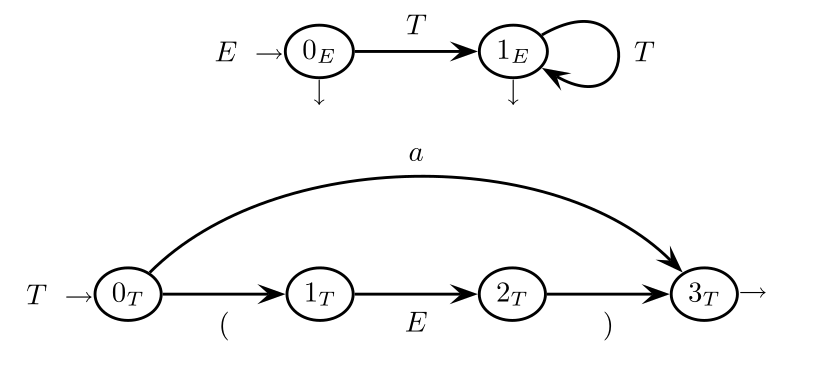
\includegraphics[width = \textwidth]{./images/exNetwork.png}
					\end{center}
				\end{figure}
				We compute the closure for candidate $\langle 0_e, \dashv \rangle$
				\begin{itemize}
					\item $\langle 0_e, \dashv \rangle$
					\item $\langle 0_t, \text{ ( }\rangle$
					\item $\langle 0_t, \text{ a }\rangle$
					\item $\langle 0_t, \dashv \rangle$
				\end{itemize}
		
		\subsection{ELR parsers}
			ELR = Extended Left to right Rightmost

			When reducing a string in input, a bottom up parser has two possible moves available: \emph{shift} to the next character (that simply means that a new 
			state is pushed on the stack and no pattern has been recognized yet) or \emph{reduce}: this means that a pattern (a right part of a rule) has been fully 
			recognized and a state can be popped from the stack. These two operations are an adapted version of the pop-push model for the memory. They also represent 
			the moving forward and backward in the rules of the grammar.

			ELR is the name for the parsers that recognize a EBNF grammar.

			To build the recognizer starting from the grammar a three-phase method has been outlined:
			\begin{enumerate}
				\item (Prerequisites: we have a network of machines that describes the grammar's rules) We build a special automaton called \emph{pilot automaton} 
				that is a generalization of the machines network. It covers all the possible combination of states and input.
				\item The pilot is inspected to check if it's suitable for deterministic parsing, and three types of failure are searched for (we'll discuss them 
				in a moment).
				\item If the test at point 2 is passed, then the DPDA is built from the pilot. 
			\end{enumerate}
			
			\subsubsection{Construction of the pilot automaton}
				The pilot automaton is (as already said) a method to represent \emph{all} the possible computational path of another one. Every state (called macro 
				state or m-state) is labeled as all the states it represents, and all the arcs keep in consideration all the possible reading for all the possible 
				states encapsulated in a single m-state.

				Every state is divided in 4 parts:
				\begin{itemize}
					\item the two (canonically) upper parts are the \emph{base} candidates: the states and lookahead characters of \textbf{non initial} state;
					\item the two (canonically) lower parts are reserved to the \emph{kernel} candidates: the states and associated lookahead of the 
					\textbf{initial} state.
				\end{itemize}
				Every final state in every m-state is usually highlighted (to help spot reductions).

				An algorithm that creates a pilot automaton can be described in this way:
				\begin{enumerate}
					\item The initial state groups the first state of the first accessed machine AND all the states of the machine that can be reached with a 
					$\epsilon$-move. (So? They're all the first states of the nonterminals that \emph{label} the outgoing arcs from the initial state. Being 
					all initial states \emph{for construction}, first m-state does not have the base part)
					\item All the other states are built in a similar way: following an arc, I add all the state that I can found to the next m-state; I select 
					the initial ones and put them in the closure, then I check for states that are reachable through a $\epsilon$-move, and also add them to the 
					closure. For the closure part, I shall recalculate the lookaheads, things that \emph{generally} I do not do with the pure base part.
				\end{enumerate}
				Is a pilot automaton still a PDA? Yes: the extra labeling of the states and the interpretation of the strings can be seen as pushing and poppoing 
				the entire candidates onto the stack and popped back when needed.
				
			\subsubsection{Meaningful example}
				We build the pilot automaton for the grammar in (5); at first glance, it can seem overly complicated, so I'll add a list of things to be noted.
				\begin{itemize}
					\item All m-states have a number of outgoing arcs that's equal to the number of outgoing arcs of \emph{all his states combined}
					\item The first state has no base part
					\item \underline{Following a path on the machine chart translates in "inheriting" the lookahead set}
					\item Watching the graph, there are two visible subsets that represents the two possible paths towards the accepting states: one in the 
					"upper level" (which has as a lookahead $\dashv$) and one in the "nested level". The first is composed of the states 
					\{$I_0$, $I_3$, $I_8$, $I_2$\} and the second one of the states \{$I_3$, $I_6$, $I_7$, $I_5$\}
				\end{itemize}
				\begin{figure}[H]
					\begin{center}
						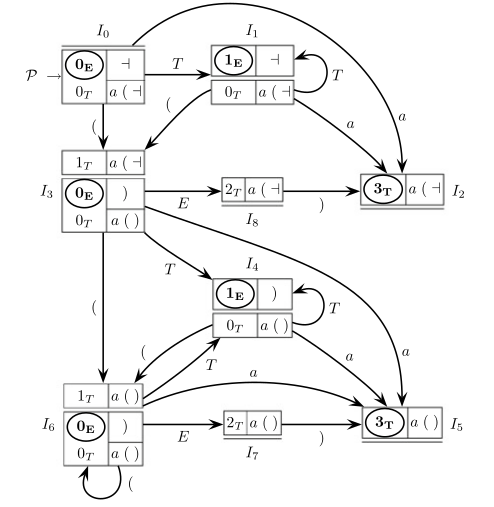
\includegraphics[]{./images/pilotAutomaton.png}
					\end{center}
				\end{figure}
				
			\subsubsection{Another meaningful example}
				Without forgetting we are at the \emph{first} step of our DPDA building, I add another good example.

				We start from this machine sets:
				\begin{figure}[H]
					\begin{center}
						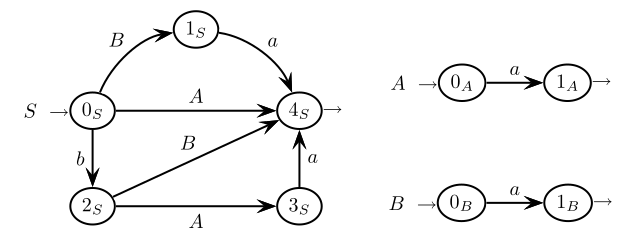
\includegraphics[width = \textwidth]{./images/ex2.png}
					\end{center}
				\end{figure}
				We derive the pilot automaton with the algorithm described above:
				\begin{figure}[H]
					\begin{center}
						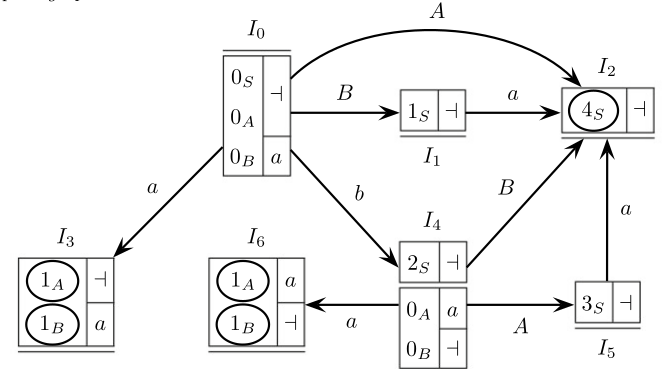
\includegraphics[width = \textwidth]{./images/ex2Pilot.png}
					\end{center}
				\end{figure}
				Again, I add a short list of things to be noted
				\begin{itemize}
					\item the first transition labeled "a" is the perfect example of \emph{following a paht makes you inherit lookaheads};
					\item m-states $I_3$ and $I_6$ represents the same states, but with different lookaheads;
				\end{itemize}
				
			\subsubsection{Deterministic check (also called ELR condition)}	
				The three possible failures in deterministic check:
				\begin{itemize}
					\item shift reduce conflicts: both a shift and a reduce are a possible in a certain configuration. This means that in a pilot automaton for all 
					the candidates $\langle q, \pi \rangle \in I$ so that q is final and for all the arcs $I \xrightarrow{a} I'$ that go out from I with terminal 
					label a it must hold that $a \notin \pi$;
					\item reduce reduce conflicts: two possible (or more) reduce paths are possible in a given configuration. In a pilot automaton, it's formulated 
					as: for all the candidate $\langle q, \pi \rangle, \langle r, \rho \rangle \in I$ that q and r are both final it must hold that 
					$\pi \cap \rho = \emptyset$;
					\item convergence conflicts: two different computations share a lookahead and a future state (this could cause reducing conflicts). This conflict 
					is the most tricky to discover, as it can only be done analyzing the graph manually: the condition to be met is something like "no different 
					states in a single m-state share a lookahead and a state".
				\end{itemize}
				
			\subsubsection{Parser algorithm}
				We focus on the implementation that makes use of a vector stack, so a LIFO memory with has also and index-like access (like vectors. You should guess 
				what a vector stack is). This enables the parser to save the exact position to return to when a reduce move is performed, accessing directly the cell 
				pointed with the saved index.

				The accepting procedure is quite obvious: the pilot automaton is traversed following the arcs when a new term is read, and reducing when the next term 
				is equal to the lookahead char in the m-state. Accepting is when we reach a final state and we only have the axiom on the stack. This procedure is an 
				incremental process: every time a m-state is leaved, on the stack are pushed all the possible candidates, and the next m-state will save the pointer 
				(index) to the previous one and so on, so that at reduce time the parser can pop off all the states from the stacks just following the indexes.

				(The official and formal way to describe the algorithm is leaved to the curious reader: page 271+ of the "Formal languages and Compilation" book from 
				Reghizzi, Breveglieri, Morzenti)
			
		\subsection{ELL parsers}
			ELL = Extended Left to right Leftmost

			ELL parsers are among the most basic top down parsers; the idea is to mimic the traversing of the machines network. The string is 
			\emph{progressively generated} using the grammar rules character by character until $\dashv$ is reached. ELL parsers relies on a stronger assumption 
			than ELRs: so that the input string can identify the rule that produces it \emph{starting from the first character}.

			The most used technique is to enrich the arcs of the pilot automaton with "guide sets" that communicate the next characters that can be encountered. 
			Relying on a stronger hypothesis means being effective in fewer cases: ELL parsers can't be built if
			\begin{itemize}
				\item Multiple transitions between states are defined. This simply means that ELL parsing isn't applicable to \emph{all} the pilot automata where 
				two or more states in the same m-state originate an arc with the same label;
				\item There are left-recursive derivation;
				\item The pilot automaton does not meet ELR condition (ELL represents a smaller set of languages). 
			\end{itemize}
			These three conditon form the \textbf{ELL condition} for automata.
			
			\subsubsection{Parser Control Flow Graph}
				A PCFG is a representation of the automata that compose the machine network that \emph{links} them all together, highlighting subsequent calls 
				and recursive dependencies. From the PCFG it's easy to derive directly the parser code.

				Starting from the machine net graph, building a PCFG means:
				\begin{enumerate}
					\item adding call arcs: these arcs connect the states that have an outgoing arc labeled as nonterminal with the first state of the machine that 
					recognizes that nonterminal;
					\item labeling call arcs: every call arc is enriched with a set of nonterminals that are the "guide set" for that call. This set of nonterminals 
					is composed of all the followers of that call:
						\begin{itemize}
							\item token that are the initials of the language generated by the submachine
							\item the empty string if the language of the subm is nullable
							\item the nonterminals that labels the subsubcalls to other submachines
						\end{itemize}
					\item enriching final states with so-called "prospect sets": prospect sets are the union of \emph{all} lookahead sets of \emph{all} the 
					occurrence of that state in the pilt automaton. This union of sets must be found watching the pilot automaton. 
				\end{enumerate}
				
				\paragraph{Example}
					We build the PCFG for the grammar in (5), so to have a continuity.
					\begin{figure}[H]
						\centering
						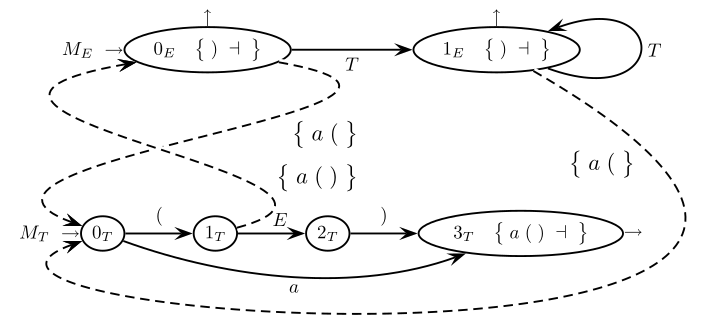
\includegraphics[width = \textwidth]{./images/PCFG.png}
					\end{figure}
			 
			\subsubsection{ELL test}
				Given the PCFG, we can easily check if an automata is ELL by exploiting a corollary of the ELL condition itself, which states that a machine network 
				satisfies ELL iff for each state, all the outgoing arcs' guide sets are disjoint. The double implication means that building the PCFG and checking 
				the disjointness of the guide sets proves if a machine network satisfies ELL or not.

				\emph{\textbf{This means we can avoid building the pilot automaton to check for ELL property}}
				
			\subsubsection{Possible implementation techniques}
				This short paragraph explains how to implement a predictive parser (but not why, tho) by means of two of the most common techniques.
				\begin{itemize}
					\item Recursive procedures: every submachine is encoded as a single procedure that scans the input tape char by char and that analyzes the input 
					token as the automaton would: guide sets and arc labels are used to build the patterns to match the current character against. Termination of a 
					subprocedure: acceptance; else an error is thrown. To recognize a nonterminal the associated procedure is called. (A lot of talking for an 
					implementation technique that's really simple in practice: just modularize the code according to the machines in the network).
					\item Explicit stack: this method does not take advantage of the recursiveness to memorize the state of the application, instead it saves it on 
					the stack directly. The parser can perform 4 different moves (here with "replace q with r" is intended pop q push r):
						\begin{enumerate}
							\item scan: if the shift arc q $\rightarrow$ r exist, then q is replaced with r.
							\item call: move performed when a submachine is invoked. Pop of the current state, push of the first state after call (so if 
							$q \xrightarrow{B} r$ replace q with r and push $0_B$), push of the first state of the called machine.
							\item return: the next character is in the prospect set of the current state, which is final: pop.
							\item recognition: if we are in the final state of the axiom machine and the current character is $\dashv$, recgnize and halt. Otherwise, 
							error and halt.
						\end{enumerate}
				\end{itemize}
				
			\subsubsection{Lookahead lenghtening}
				Often it's sufficient to increase the lenght of the lookahed (to more than one token) to render a top down parser deterministic fom a non-ELL grammar. 
				In this course, the only method is a "eagle eye" one where you spot the perfect lenght just looking at the PCFG and choosing which minimum lookahed 
				set grants determinism, basing yourself on pure parser instinct.
				
		\subsection{Earley algorithm}
			The Earley algorithm is a method to recognize strings from a grammar even if this is ambiguous. The pseudocode approach both the book and the slides take 
			is very counterintuitive, in my opinion. So, I will try just to explain \emph{how practically} a Earley recognizers is built and used. Keep in mind that 
			this procedure should build \emph{a software}.

			First, initialize the vector of candidates to E = \{ $\langle 0_s, 0 \rangle$ \} that represent the initial state and the first value

			Then, with $n$ taken as the lenght of the string to recognize, we initialize all the elements of E[1..n] to the empty set.

			We complete the first element E[0]. Completing an element (applying the \emph{completion} operation to it) means computing the closure of the state (and 
			adding to the E[i] set of candidates the closure's states) and calculating also all the states that are reachable through a nonterminal shift (watch out: 
			with nonterminal shift we are referring to the operation of "arriving on E[i] with a nonterminal shift", not leaving this state), adding them also to the 
			state.

			We then compute, for every token in the string, the \emph{terminalshift} for every element in the vector (terminalshift means nonterminalshift with 
			terminal symbols. For every candidate in previous state that can terminalshift to a candidate in the current state add that transiction [represented as 
			the candidate $state, index - 1$] to this vector element) to build the shifting operation, then we complete it.

			This algorithm is similar to the method to build a pilot automaton, but instead of lookahed sets just the position in the vector of the caller state is 
			memorized. The string is accepted if the last element of the vector is of type $\langle finalstate, 0 \rangle$: this means that the condition is 
			accepting (finalstate) and the whole string is accepted (0).
			
			These example and notation should clear all remaining doubts:
			\begin{figure}[H]
				\centering
				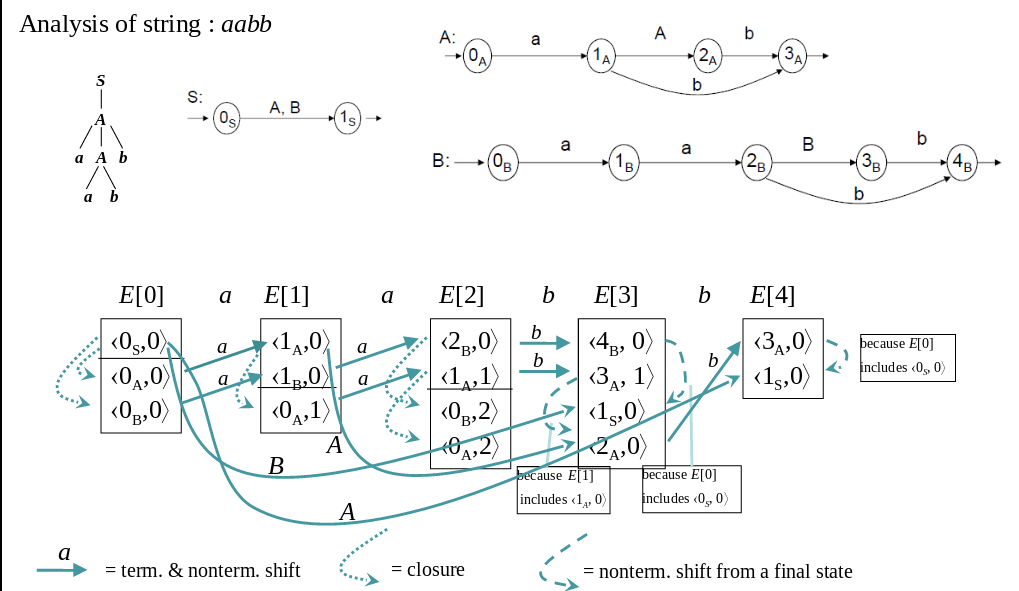
\includegraphics[width = \textwidth]{./images/exEarley.png}
			\end{figure}